\section{The Interlaken Protocol}
\label{sec:interlaken}

After the survey of available protocols and their specifications, the Interlaken protocol appeared as the one meeting nearly all requirements in contrast to the other surveyed protocols~\cite{InterlakenAlliance}. Not only the specifications looked propitious for the current situation but the documentation also offered lots of information which made it a lot clearer how the protocol functions and how to possibly realize this in hardware.

Until now the Interlaken Protocol has been described in short but this section will be dedicated to a more extended description of the Interlaken protocol.
As described earlier the protocol can be divided into different components which belong in their specific OSI layer. A complete Interlaken frame is formed in the first two OSI layers. The frame itself containing the data and control words is formed in the second layer while the first layer adds the three bit preamble that comes with the encoding.

\subsection{Overview} 
	This section will present a complete overview to clear up how the protocol is structured and in what order the functions will be discussed. The earlier presented Figure \ref{fig:protocol_overview} can be used as reference in this case. The Interlaken also functions is this order but the blocks get somewhat complexer. 

	\begin{figure}[H]
		\centering
		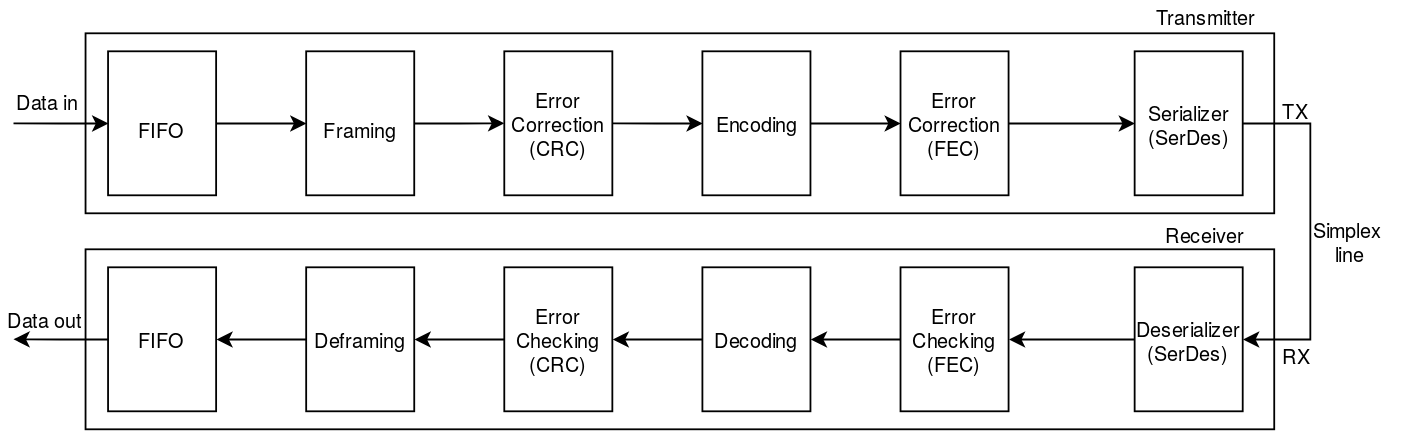
\includegraphics[width=\textwidth]{Protocol_Overview.png}	
		\repeatcaption{fig:protocol_overview}{Protocol overview.}
	\end{figure} 
	
	Interlaken uses two ways of framing which both add control words. First bursts will be formed by adding framing words and these will be covered by the first CRC and after this the meta frame will be formed which will be covered by another CRC. This can be interpreted as the framing and error correction blocks repeating once. 
	Because of this the control word itself will be explained first and after this the two ways of framing will be discussed in more detail. Flow control and it's supported variants will also be described. This will be followed by the CRC variants Interlaken makes use of since all components containing CRC have been described. 
	
	The encoding will consist of a scrambler and the 64b/67b encoder itself which will be described respectively. FEC is available as an extension and will not be described yet since it is not included in the standard protocol description.


\subsection{Control Word Format}
	\label{subsec:interlaken_controlword}
	It is essential to know how the control word is structured to understand how Interlaken handles data transmission. There are two different types of control words used depending on the control bit status. In case this is a one it concerns an idle/burst control word and in case this is a zero it concerns a framing layer control word. Figure \ref{Fig:Interlaken_ControlWord} depicts the word formats~\cite{InterlakenProtocol}.
	
	\begin{figure}[H]
		\centering
		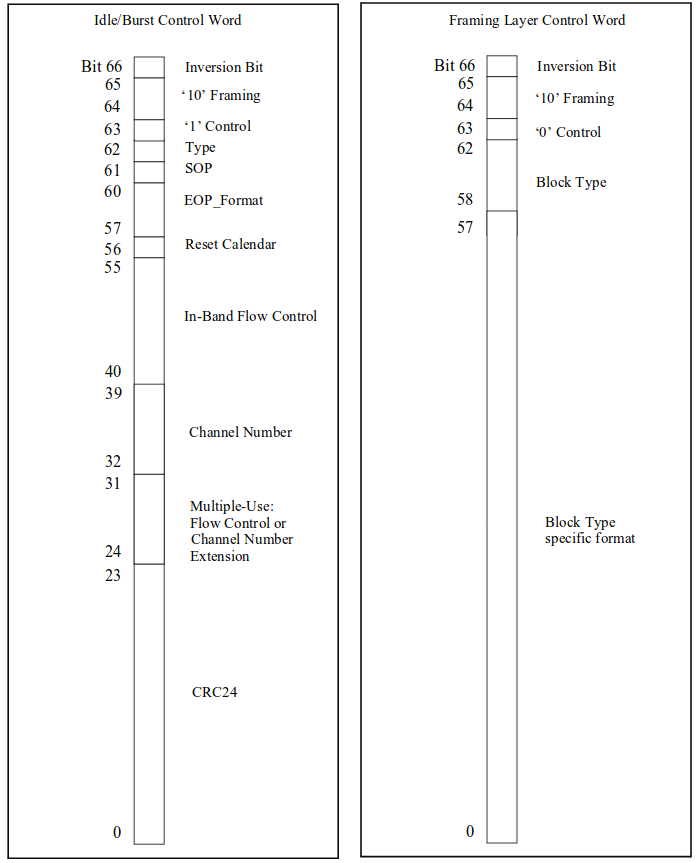
\includegraphics[width=0.75\textwidth]{Interlaken_ControlWord.png}	
		\caption{Interlaken control word formats.}
		\label{Fig:Interlaken_ControlWord}
	\end{figure}
	
	As seen the two idle/burst control words contain a type bit which indicates whether the word is an idle or burst word. It includes Start and End Of Packet (SOP and EOP) indicators which will be explained later. Flow control and CRC are also present in this word and there is space for the specific channel number in the case of bonding. \\
	
	The framing word has a less complex structure and contains a block type field which functions as an identification. After this the specific format according to the block type itself will follow. The structure of this last data block differs for each type and this will be explained further in section \ref{subsec:interlaken_metaframe}. \\
	
	For the sake of clarity Figure \ref{Fig:Interlaken_WordStructures} contains a diagram which depicts all word types and shows how they are distinct from each other. This makes it easier to distinguish the words in one overview compared to repeatedly looking up the images and tables depicted in the Interlaken documentation.
	
	\begin{figure}[H]
		\centering
		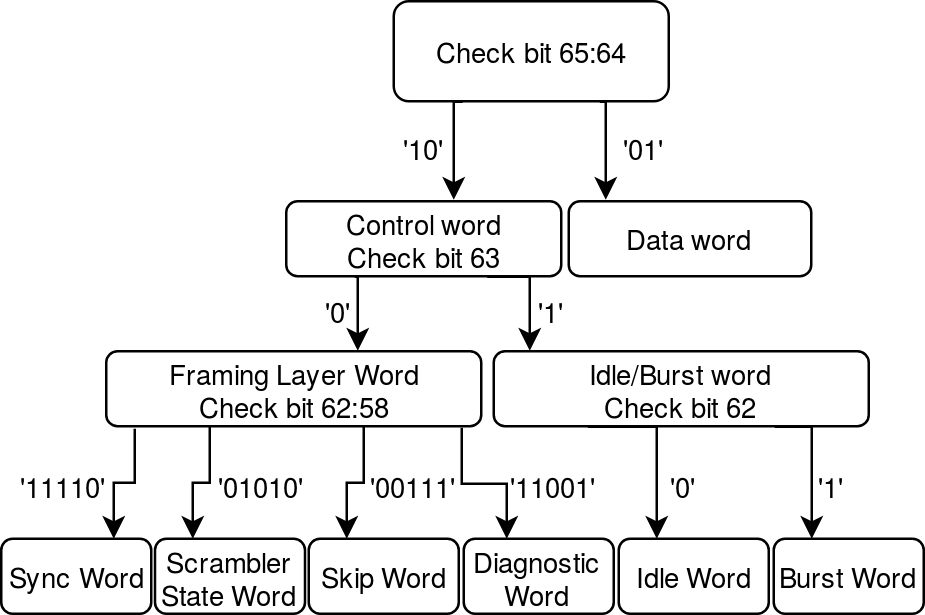
\includegraphics[width=0.8\textwidth]{Interlaken_WordStructures.png}	
		\caption{A complete overview of word types and their structure.}
		\label{Fig:Interlaken_WordStructures}
	\end{figure}
\newpage


\subsection[Bursts]{Bursts \hfill OSI Layer 2}
	\label{subsec:interlaken_bursts}
	The Interlaken interface is designed to transmit data in packets. Incoming data will firstly be packed in so called bursts which are of a specific length. The burst will always start with a control word containing the Start Of Packet (SOP) bit set. After this the data will follow and the burst will end with a control word containing the End Of Packet (EOP) bit set. This is only the case when data can be packed in a single burst. In case the amount of data to be transmitted is greater than the data that fits in a single burst of maximum length, multiple bursts will be transmitted with control words in between to still keep the data in separate bursts. These words will have neither the SOP or EOP bits set.\\
	
	In case the to be transmitted data consists of less bytes than the minimum amount required for a burst, this won't cause problems. The first part of the burst will be filled up with the data. After it a control word with the EOP bit set will follow and the other bytes will be filled with idle words to reach the minimum burst length. This situation is depicted in Figure~\ref{Fig:Interlaken_Burst}~\cite{InterlakenProtocol}. A total of 72 bytes have to be transmitted and the maximum burst length is 64 bytes so the first burst is completely filled. The burst after it will contain the last 8 bytes but this is not enough to fill the minimum length of a burst. So the first eight bytes will be put in a burst pack and the other required bytes are filled with idle words. In this case the first idle word will contain the EOP bit set.
	
	\begin{figure}[H]
		\centering
		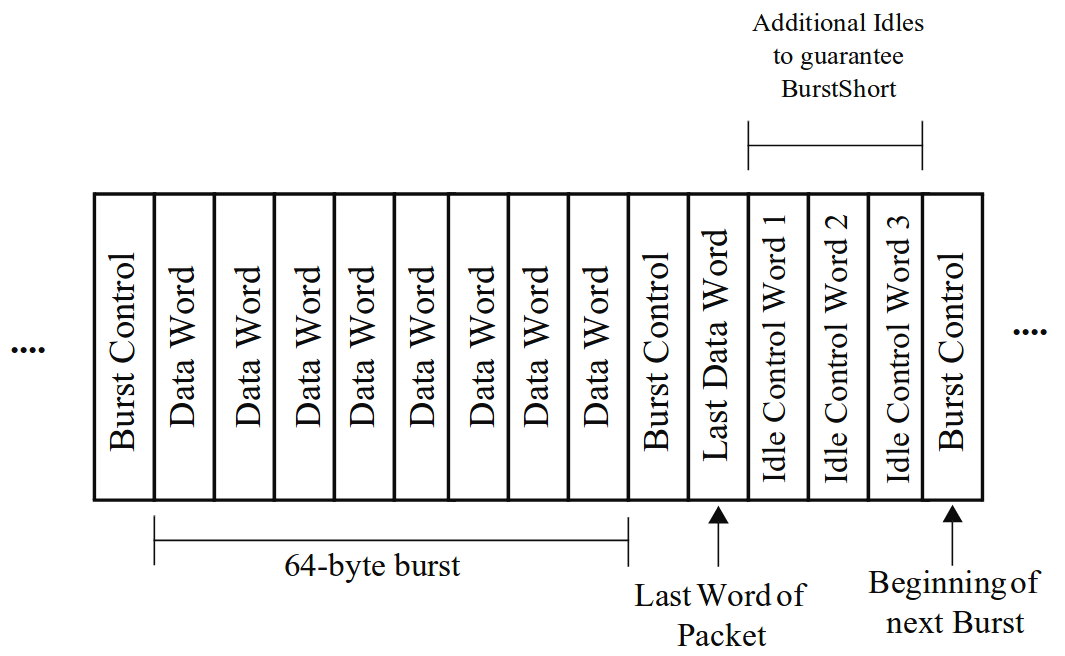
\includegraphics[width=0.7\textwidth]{InterlakenBurst.png}	
		\caption{An example of a short burst.}
		\label{Fig:Interlaken_Burst}
	\end{figure}
	
	The maximum recommended size of the bursts which is mentioned as BurstMax contains 256 bytes. The minimum recommended size of a burst is 32 bytes and is known as BurstShort~\cite{InterlakenRecommendations}. Every byte amount in between can also be transmitted, this has to be an eight byte increment of course since the data packs are all 64-bit. BurstMax and BurstMin can be configured by the designer who implements the burst controller.\\
	
	Unfortunately a lot of bandwidth is wasted in case idle words are added. A solution for this complication is mentioned in the Interlaken documentation. An additional variable BurstMin is introduced which in size is half that of BurstMax and is bigger or equal to BurstShort. When the payload to be sent is bigger than BurstMax but smaller than BurstMax plus BurstShort this means that too much idle words will be used again. So in this case a payload of BurstMax minus BurstMin will be sent. This way it can be guaranteed that the last data to be transmitted is enough to fill up BurstShort.
	
	In the same case of the 72 byte transmission it is now possible to prevent the presence of idle words. The total to be transmitted data is smaller than BurstMax and BurstMin summed and bigger that BurstMax alone so two transmission bursts are required. Burstmax and BurstMin are assigned a value of 64 and 32 bytes respectively. The solution is simple by deciding the first burst will contain BurstMax-BurstMin bytes, so 32 bytes will be packed. After this 40 bytes are still remaining and will be transmitted in a burst without the necessity of idle words. The bursts are visualized in Figure~\ref{Fig:Interlaken_Burst2}. \\
	
	\begin{figure}[H]
		\centering
		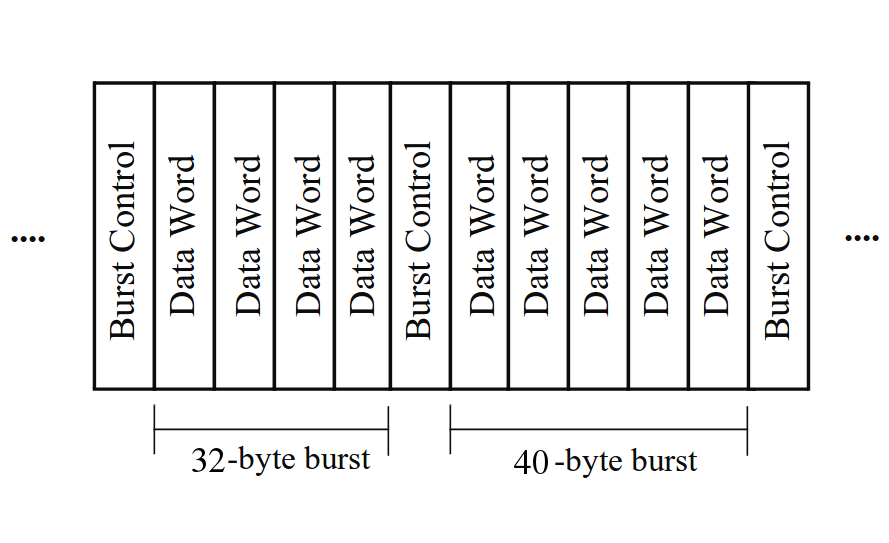
\includegraphics[width=0.6\textwidth]{InterlakenBurstGud.png}	
		\caption{An example of a burst without idles.}
		\label{Fig:Interlaken_Burst2}
	\end{figure}
	
	As seen this results in a significant reduction of wasted bandwidth. In the first example fifteen packets were transmitted including the idle words. With the optimization added this occupied size has been reduced to 12 packets which saves 24-bytes or 20\% of bandwidth.\\
	
	Another important aspect is that data and control integrity is ensured by the generation of a 24-bit CRC. The control word which follows the data will contain the CRC24. All data words the burst contains and the control word itself will be covered by the CRC24.
\newpage


\subsection[Meta Frame]{Meta Framing \hfill OSI Layer 2}
	\label{subsec:interlaken_metaframe}
	The Interlaken Protocol introduces a way of framing using the term Meta Frame. This introduces four control words which are used in combination with the payload to form a complete frame containing essential information for the receiver. The payload in this case is the data which was packed in bursts while Synchronization, Scrambler State, Skip and Diagnostic words are added. The structure of a Meta Frame is visualized in Figure~\ref{Fig:Interlaken_MetaFrame}.
	
	\begin{figure}[H]
		\centering
		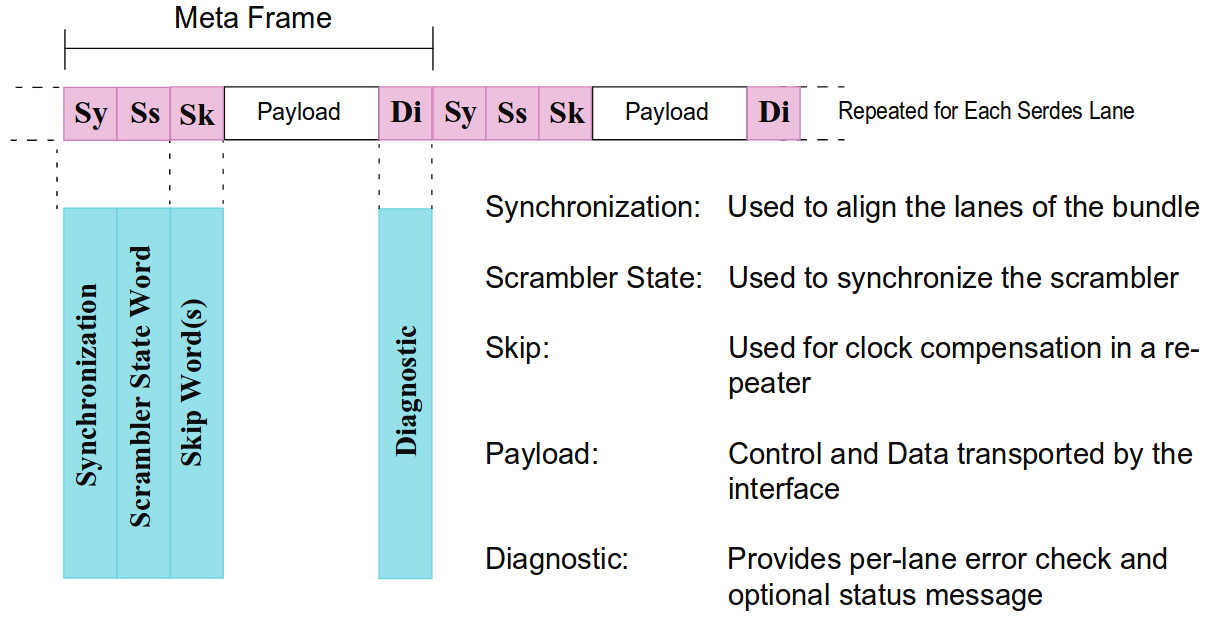
\includegraphics[width=0.8\textwidth]{Interlaken_Meta.png}	
		\caption{Interlaken Meta Frame structure.}
		\label{Fig:Interlaken_MetaFrame}
	\end{figure}
	
	The total amount of bytes the Meta Frame contains is fully configurable and using a variable called MetaFrameLength. However an amount of 2048 words is recommended by the Interlaken Alliance~\cite{InterlakenRecommendations}. This also includes the Synchronization, Scrambler State, Skip and Diagnostic words. It is also mentioned that this frame length is a real limit, so the meta framer doensn't wait for a burst to finish. The framing words can appear at any moment during a burst. This also indicates the components responsible for generating the bursts and meta frames don't have to communicate about this.
	The control words and their block types are shown in Figure~\ref{Fig:Interlaken_BlockTypes} and will be explained in their own dedicated sections.
	
	\begin{figure}[H]
		\centering
		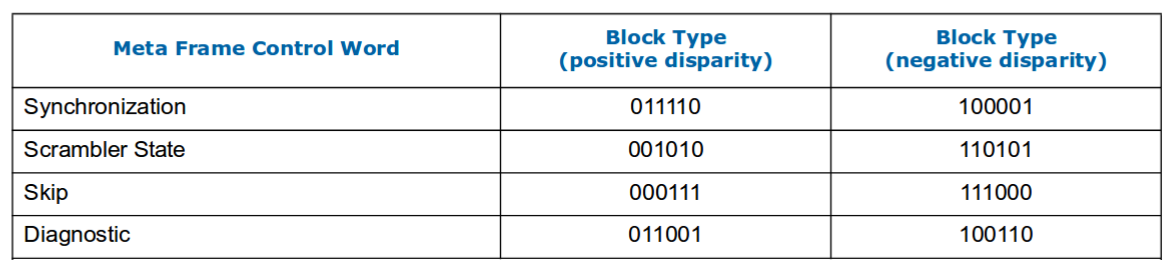
\includegraphics[width=0.8\textwidth]{Interlaken_BlockType.png}	
		\caption{Interlaken framing layer block types.}
		\label{Fig:Interlaken_BlockTypes}
	\end{figure}
	
	While the Meta Frame control words take up a total bandwidth of 32-bytes every frame, this doesn't really increase the amount of overhead since they appear infrequently. When for example the length of a Meta Frame is chosen to be the recommend size of 2048 words, 2044 of these words will effectively carry the payload. Leaving generated overhead by the bursts out of account, this results is an overhead of about 0,2\%.
	
	\subsubsection{Synchronization and Scrambler State}
	The synchronization and scrambler state words are unique in the aspect they are the only words that must be transmitted unscrambled. The synchronization word is a static word both known to the transmitter and receiver. One of it's purposes is to lock the scrambler and literally synchronize the transmitter and receiver. After receiving the 4th consecutive synchronization word, the scrambler is locked and can descramble data. 
	
	Another purpose of the synchronization word is to align multiple lanes in case channel bonding is used. The sync word will be transmitted simultaneously on all lanes and the receiver recognizes these words and will measure the skew between all lanes. Interlaken also features additional logic which can be adjusted to compensate for skew across lanes so all data lanes will be aligned nearly perfectly. Unfortunately Interlaken doesn't describe this logic and the implementation is left to the designer. A visual representation can be seen in Figure~\ref{Fig:Interlaken_LaneAlignment}.
	
	\begin{figure}[H]
		\centering
		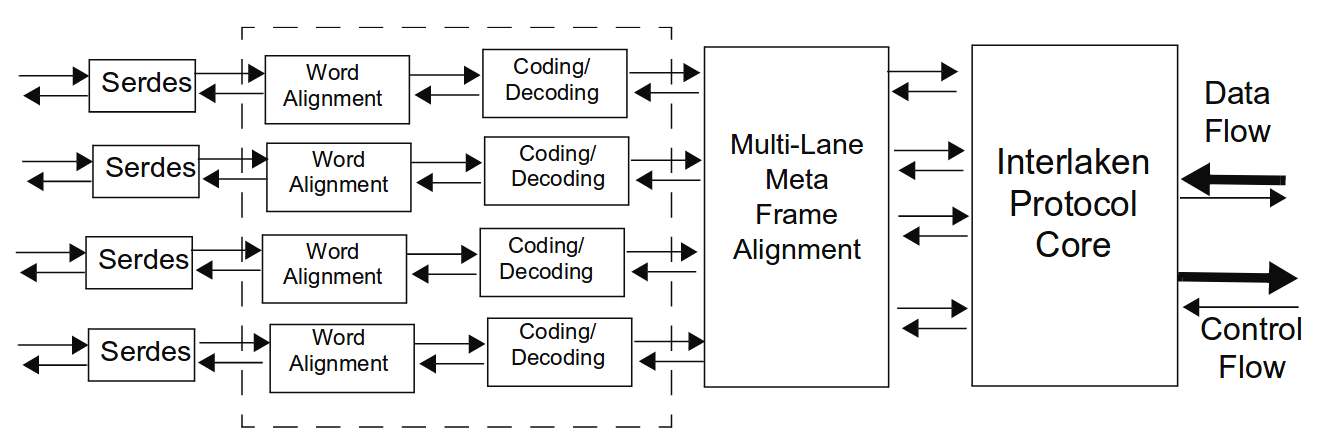
\includegraphics[width=0.8\textwidth]{Interlaken_LaneAlignment.png}	
		\caption{Interlaken lane alignment.}
		\label{Fig:Interlaken_LaneAlignment}
	\end{figure}
	
	The scrambler state word is used to compare the current state of the receiving side scrambler to the state it has to be according to the transmitter. When these words match, all data has been descrambled correctly. If this is not the case something went wrong and this will result in an error after three consecutive mismatches. This will also cause the scrambler to lose it's lock and to reset.
	
	The synchronization word containing it's valid pattern and scrambler state word are shown in Figure~\ref{Fig:Interlaken_SyncScramWords}.
	
	\begin{figure}[H]
		\centering
		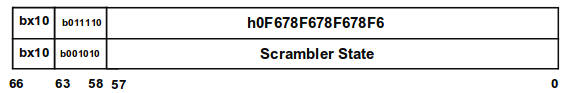
\includegraphics[width=0.7\textwidth]{Interlaken_SyncScramWord.png}	
		\caption{Interlaken synchronization and scrambler state words.}
		\label{Fig:Interlaken_SyncScramWords}
	\end{figure}
	
	\subsubsection{Skip Word}
	The skip word is used enable to the ability of clock compensation in case a repeater stands in between the transmitter and receiver. The clock rate can slightly differ on each side of the repeater which results in corrupt data on the receiving side. Adding skip words is very useful in this situation because these can later be removed by the repeater or more skip words can be added. This way the differing clock rate can be compensated. 
	
	The structure of a skip word is depicted in Figure~\ref{Fig:Interlaken_SkipWord} and as seen this contains just a static package of bits. Skip words can be placed nearly anywhere is the complete Meta Frame. Except in between the diagnostic, synchronization and scrambler state words. It is also possible to add multiple skip words at different positions in the Meta Frame.
	
	\begin{figure}[H]
		\centering
		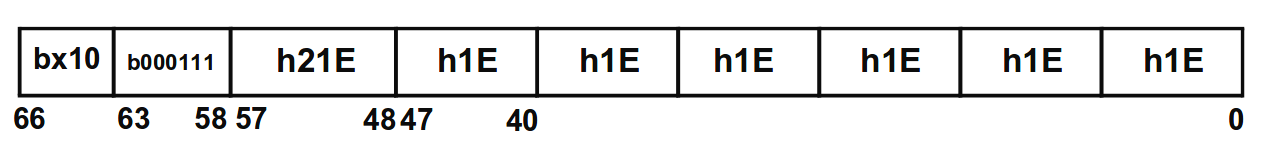
\includegraphics[width=0.7\textwidth]{Interlaken_SkipWord.png}	
		\caption{Interlaken skip word.}
		\label{Fig:Interlaken_SkipWord}
	\end{figure}
	
	\subsubsection{Diagnostic Word}
	This word type is meant to indicate the current lane status and offers error correction for the lane this message is received on. The diagnostic word structure is depicted in Figure~\ref{Fig:Interlaken_DiagWord}.
	
	\begin{figure}[H]
		\centering
		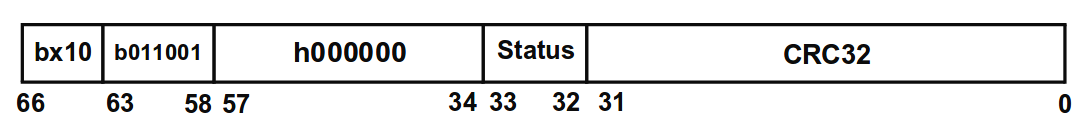
\includegraphics[width=0.7\textwidth]{Interlaken_DiagWord.png}	
		\caption{Interlaken diagnostic word.}
		\label{Fig:Interlaken_DiagWord}
	\end{figure}
	
	The 2-bit Status field contains two different messages. One bit indicates the health of this lane and the other bit represents the health of the entire interface. When the bits are high this indicates a healthy interface while a low bit gives indication a problem occurred.\\
	
	Error-correction is added in the form of a 32-bit CRC. So every diagnostic word contains a CRC-32 field which covers all previous data and the diagnostic word itself. More detailed information will be present in section~\ref{subsec:interlaken_CRC}.
\newpage


\subsection[Flow Control]{Flow Control \hfill OSI Layer 2}
	\label{subsec:interlaken_flowcontrol}
	Interlaken provides documentation on multiple ways of flow control that can be implemented. Communication will be through per-channel backpressure. This indicates that the receiver will hold off the transmitting device on sending packages in case no more data can be processed. When the receiver has solved the problem transmission can continue where it left off. This can occur in case the receiving buffer is nearly completely filled or the receiver lacks processing power. Out-of-Band, In-Band and Full-Packet Flow Control are featured by Interlaken.
	
	A so called calendar can be used in the case of flow control. This is simply a structure to which channels may be mapped. It can be used to map the flow control to any set of calendar entries or to provide link-level flow control. In the last case a binary one would mean permission to transmit data (XON) and a zero would indicate transmission has to cease immediately (XOFF).
	
	\subsubsection{Out-of-Band Flow Control}
	An Out-of-Band Flow Control option is defined to support systems that require simplex operation. So in case data flows only in one direction. To overcome this and still feature flow control, a separate channel is required. This can be made possible by an extra physical connection and the advantage of this technique is that the full bandwidth is available on the main data transmission channel. 
	
	The interface makes use of three signals. A clock, the flow control data and a synchronization indicator. Figure \ref{Fig:Interlaken_FC_Out-of-Band}\cite{InterlakenProtocol} shows a visual representation of this. The data is synchronized to the clock signal while the separate synchronization signal indicates the start of a new calendar.
	
	\begin{figure}[H]
		\centering
		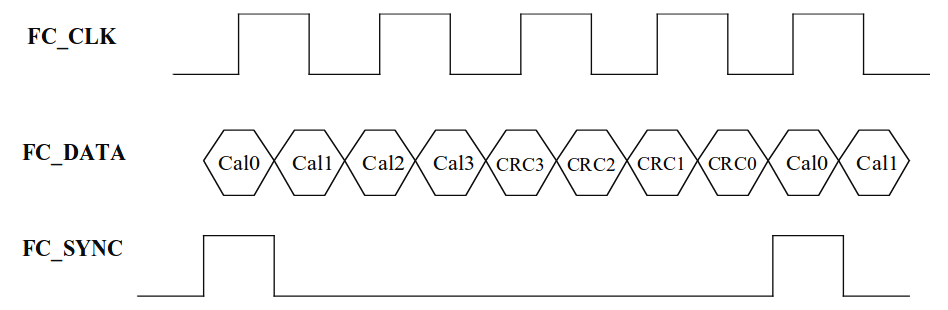
\includegraphics[width=0.7\textwidth]{Interlaken_FC_Out-of-Band.png}	
		\caption{Interlaken Out-of-Band Flow Control timing diagram.}
		\label{Fig:Interlaken_FC_Out-of-Band}
	\end{figure}
	
	In this case a 4-bit calendar is used but this of course depends on the number of channels implemented. To ensure flow control data integrity a 4-bit CRC is used which section~\ref{subsubsec:interlaken_CRC-4} will discuss in more detail.
		
	%Since Interlaken already reserves space in the control words for Flow Control this doen't offer extra bandwidth.
	
	\subsubsection{In-Band Flow Control}
	This makes use of the data channel to transmit the flow control status. This is an option provided for systems that support full-duplex operations and saves physical connections. The flow control calendar will be moved to the space in the idle/burst control words which is intended for this use.
	
	There are 16-bits available but the 8-bit multi-use field can also be used for flow control which brings the total amount of usable bits to 24. The reset calendar bit is available to synchronize the moment at which the calendar starts. In case this bit is not set, the calendar will not be reset and continue where it left off in the previous control word.
	
	Since the idle/burst control words are covered by the CRC-24 this will render the earlier mentioned CRC-4 unnecessary to implement.
	
	\subsubsection{Full-Packet Flow Control}
	This way of flow control is optimized for usage while complete package transmissions, without any interleaving, are required. Two interpretations of the full-packet mode flow control are given. 
	
	The first method is to stop the transmission immediately after receiving the XOFF message. This reduces the required size of the receiving buffer but causes head-of-line blocking of other channels.
	
	The second interpretation is to finish the current packet before stopping the transmission. This increases the required buffer size and prevents head-of-line blocking of channels.
	
	It is possible to choose one of the two interpretation but is also possible to combine them in a way if required. This depends on what kind of behavior the application requires.
	
\newpage


\subsection[CRC generation]{CRC generation \hfill OSI Layer 2}
	\label{subsec:interlaken_CRC}
	Interlaken covers different parts of the to be transmitted data with separate CRC polynomials. This subsection will be dedicated to how the CRC's have to be generated according to the Interlaken documentation and which part of the transmitted data they will cover. \\
	
	The generation of an n-bit CRC will start with the polynomial being reset to all ones. After this the data stream will enter the component and thus generate the CRC. This will be sent to the CRC function with the MSB of the bytes always entering first. When this is done, the polynomial will be inverted and moved to the reserved space in the right bit order. To keep things consistent the CRC will be moved using the same format as the data itself.\\
	
	Three different CRC polynomials are documented by the Interlaken protocol. This concerns a 4-bit, 24-bit and 32-bit polynomial. The next sections will provide more information on what data they will cover, how they will be calculated and what polynomial will be using.
	
	\subsubsection{CRC-4}
	\label{subsubsec:interlaken_CRC-4}
	Out-of-band flow control data integrity is ensured by a 4-bit CRC generation. This covers up to 64 bits of data used for flow control. The polynomial chosen for this CRC variant is 0x0D in hexadecimal form. The complete polynomial in equation form is also written down.
	\begin{equation*}
		X^{4}+X+1
	\end{equation*}
	
	In case In-Band Flow Control is used this 4-bit CRC won't be necessary since the Flow Control information will then be included in the Idle/Burst words.
	
	\subsubsection{CRC-24}
	\label{subsubsec:interlaken_CRC-24}
	The data bursts will be covered by a 24-bit CRC. The data packets and the control word itself will be covered. The Idle/Burst control words contain a reserved space where the generated CRC-24 can be moved to. Of course the CRC field will be padded with zeros while the CRC is being generated.
	
	The polynomial of CRC-24 can be written out as 0x328B63 in hexadecimal form. The equation below represents the complete polynomial.
	
	\begin{equation*}
		X^{24}+X^{21}+X^{20}+X^{17}+X^{15}+X^{11}+X^{9}+X^{8}+X^{6}+X^{5}+X+1
	\end{equation*}
	
	\subsubsection{CRC-32}
	\label{subsubsec:interlaken_CRC-32}
	The Meta Frame will be covered by a 32-bit CRC. This will cover the complete payload in a frame and the Synchronization, Scrambler State, Skip and Diagnostic words. Since the CRC-32 will be included in a Diagnostic word at the same frame that has been covered, the bits of where the CRC-32 will be placed have been padded with zeros.
	The Scrambler State word will also be filled with zeros since generating the CRC has to happen before scrambling the data. Framing bits will of course also be excluded since these have not been added yet and this is really meant to check the data itself.
	
	The CRC-32 is generated for every individual lane which offers the advantage that errors can be traced to a specific lane in case channel bonding is implemented. This could prove a very useful feature in case one of the lanes will cause error's since it is immediately clear which lane is the cause.
	
	The polynomial Interlaken uses for the implementation of CRC-32 is 0x1EDC6F41 in hexadecimal format. The complete polynomial in equation form is also written out.
	
	\begin{displaymath}
		\resizebox{\textwidth}{!} {
		$X^{32}+X^{28}+X^{27}+X^{26}+X^{25}+X^{23}+X^{22}+X^{20}+X^{19}+X^{18}+X^{14}+X^{13}+X^{11}+X^{10}+X^{9}+X^{8}+X^{6}+1 $ }
	\end{displaymath}
	
	A visual representation of the CRC-32 calculation can be seen in Figure~\ref{Fig:Interlaken_CRC32}. The Scrambler State words and placeholder for the CRC-32 will be padded with zeros while the CRC is generated.
	
	\begin{figure}[H]
		\centering
		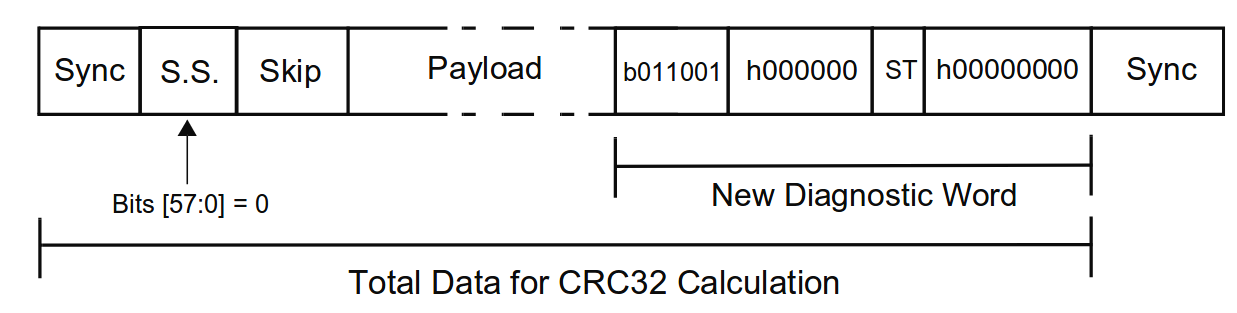
\includegraphics[width=0.7\textwidth]{Interlaken_CRC32.png}	
		\caption{Interlaken CRC-32 calculation.}
		\label{Fig:Interlaken_CRC32}
	\end{figure}
\newpage


\subsection[Scrambler]{Scrambler \hfill OSI Layer 1}
	While other protocols may choose to implement a self-synchronous scrambler, the Interlaken protocol makes use of an independent synchronous scrambler. A self-synchronizing scrambler offers the great advantage it doesn't require constant synchronization but this comes with a disadvantage. When an error occurs the scrambler will replicate this error multiple times because it makes use of two feedback taps. This way even correct data will arrive corrupted at the receiving side which is absolutely undesirable. This is the primarily reason Interlaken has implemented another form of scrambling. The independent synchronous scrambler merely uses multiple XOR gates to generate output data. \\
	
	The scrambler make use of a 58-bit polynomial which is visible beneath and accepts a 64-bit input. The polynomial can be interpreted in hexadecimal value as 0x400008000000000.
	
	\begin{displaymath}
	X^{58}+X^{38}+1
	\end{displaymath}
	
	The polynomial is activated after resetting the device and won't have to be reset anymore. This also makes clear why the scrambler state word has to be transmitted at the start of each Meta Frame. The current state of the polynomial will be compared to the state it should be according to the transmitter. This way it can be ensured the descrambled data is identical to the data before scrambling at the transmitter side. \\
	
	All to be transmitted words will be scrambled except for the synchronization and scrambler state words. In this case the scrambler will be put on hold and the polynomial state won't change since these words have to be transmitted unscrambled. When the descrambler starts after a reset, the first scrambler state word should be used to descramble the incoming data. This is also one of the reasons these two words have to be transmitted unscrambled, otherwise they can't be read because the descrambler is not yet synchronized for the first time or there is a chance they will be descrambled to an incorrect word and there is no way to detect mistakes in the descrambler state. \\
	
	It is recommended to reset all scrambler states to a different value on each lane. This minimizes the cross-talk between lanes but this choice is up to the designer. While this is important for the transmitting side, it is not necessary to transmit the reset state to the receiver since short after this reset the scrambler state will be send to synchronize the scrambler and descrambler.
\newpage


\subsection[Encoder]{Encoder \hfill OSI Layer 1}
	Interlaken makes use of the 64b/67b encoding as already explained in subsection~\ref{subsec:64b67b}. Two of these bits will indicate the presence of a data or control word like used in the 64b/66b encoding. The third bit or actually last by of the encoded packet will cause an inversion of the complete word when set. It is clearly documented in the Interlaken Protocol Definition that 64b/66b encoding completely relies on the scrambler in case of DC-balancing. This comes which the risk of unwanted increases in the bit-error rate after certain time periods. An excellent solution to prevent the occurrence of these disadvantages is to use 64b/67b encoding. One bit additional overhead is added but excellent DC balance will be provided. It is important to know that in high speeds communications timings often won't allow a full voltage swing before the next bit is transmitted so causing DC unbalance is done fairly quick.\\
	
	The encoder keeps track of the running disparity in data packets. When the incoming binary data contains a logic one the disparity will be incremented by one and when the data contains a logic zero the disparity will be decremented by one. This will also be done for the new data following up this packet. In case both data packets contain averaged more ones or zeros then the new data will be inverted to balance the average amount of ones and zeros thus canceling possible DC unbalance. The encoder will always try to keep the running disparity within a +/- 96-bit boundary. The complete preamble used by the 64b/67b encoder is depicted in Figure~\ref{Fig:Interlaken_EncoderPreamble}~\cite{InterlakenProtocol}. Every lane keeps track of it's own running disparity.
	
	\begin{figure}[H]
		\centering
		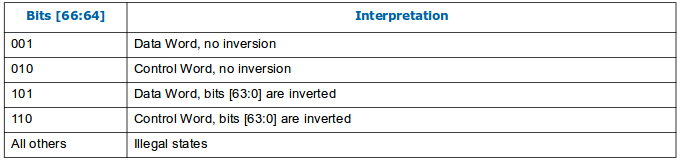
\includegraphics[width=0.7\textwidth]{Interlaken_EncoderPreamble.png}	
		\caption{Preamble of the 64b/67b encoding used in the Interlaken protocol.}
		\label{Fig:Interlaken_EncoderPreamble}
	\end{figure}
	
	The encoder gains lock after 64 consecutive legal sync headers appear at the same position in the incoming data. Since the preamble is 3-bit which offers eight possibilities but only four of them are legal, the occurrence of incorrect sync will be very low.
	Of course the occurrence of illegal states are possible. If these conditions appear multiple time the encoder will lose it's lock or won't lock.
\newpage
